\documentclass[12pt]{report}

\usepackage[francais]{babel}
\usepackage[utf8]{inputenc}
\usepackage[T1]{fontenc}
\usepackage{amsmath}

\usepackage[cyr]{aeguill}
\usepackage{fancyheadings}
\usepackage[pdftex]{graphicx}
\DeclareGraphicsExtensions{.jpg,.pdf,.png}
\usepackage[pdftex,colorlinks=true,linkcolor=blue,citecolor=blue,urlcolor=blue]{hyperref}
\usepackage{anysize}
\marginsize{22mm}{14mm}{12mm}{25mm}
\usepackage{natbib}
\usepackage{icomma}


\begin{document}
\pagestyle{fancyplain}
\renewcommand{\chaptermark}[1]{\markboth{\chaptername\ \thechapter. #1}{}}
\renewcommand{\sectionmark}[1]{\markright{\thesection. #1}}
\lhead[]{\fancyplain{}{\bfseries\leftmark}}
\rhead[]{\fancyplain{}{\bfseries\thepage}}
\cfoot{}

%% Voilà mes légendes de figures comme je les aime :
\makeatletter
\def\figurename{{\protect\sc \protect\small\bfseries Fig.}}
\def\f@ffrench{\protect\figurename\space{\protect\small\bf \thefigure}\space}
\let\fnum@figure\f@ffrench%
\let\captionORI\caption
\def\caption#1{\captionORI{\rm\small #1}}
\makeatother

\graphicspath{{img/}}

%%%%%%%%%%%%%%%%%%%%%%%%%%%%%%%%%%%%%%%%%%%%%%%%%%%%%%%%%% Couverture :
\thispagestyle{empty}
{\Large
\begin{center}
Luc LAPORTE
\vskip1cm

%% Pour redéfinir la distance entre la boite et le texte
\fboxsep6mm
%% Pour redéfinir l'épaisseur de la boite
\fboxrule1.3pt

%% Le \vphantom{\int_\int} sert à introduire de l'espace entre les deux lignes
%% (essayez donc de le commenter)
$$\fbox{$
  \begin{array}{c}
  \textbf{Titre}
  \vphantom{\int_\int}
  \end{array}
  $}
$$
\end{center}
\vskip8cm

\begin{flushright}
\textit{Encadrant :}

Zacharie ALES
\end{flushright}
}

\clearpage

%%%%%%%%%%%%%%%%%%%%%%%%%%%%%%%%%%%%%%%%%%%%%%%%%%%%%%%%%% Table des matières :
\renewcommand{\baselinestretch}{1.30}\small \normalsize

\tableofcontents

\renewcommand{\baselinestretch}{1.18}\small \normalsize


%%%%%%%%%%%%%%%%%%%%%%%%%%%%%%%%%%%%%%%%%%%%%%%%%%%%%%%%%% Introduction :
\chapter{Introduction}

\section{Problème de set-cover}

\subsection{Définition du problème}

Soit un ensemble U, un sous-ensemble de l'ensemble des parties de U, et un entier k. On souhaite savoir si il existe un sous-ensemble T de S de taille k tel que tous les éléments de U sont couvert par l'union des sous-ensemble de T, c'est-à-dire :
$$
\forall e \in U, \ e \in \underset{t \in T}{\cap}t
$$

\subsection{Résolution sous la forme d'un programme linéaire}

Résoudre ce problème revient à résoudre le programme linéaire suivant:

$$
\left\{
    \begin{array}{ll}
        min &  \underset{s \in S}{\sum}x_s \\
        tq &  \underset{s , \ e\in s} {\sum}x_s \ge 1, \ \forall e e \in U \\
         & x_s \in \{ 0,1 \}, \ \forall s \in S
    \end{array}
\right.
$$
La fonction coût à optimiser correspond à la taille du sous-ensemble T que l'on cherche à minimiser, la première contrainte impose que tout les éléments de U sont couverts par l'union des sous-ensembles de T. La dernière contrainte impose que l'on peut soit choisir un sous-ensemble dans la couverture, soit ne pas le prendre.

\subsection{Application du problème de set-cover}

Le problème de set-cover trouve une application dans la résolution du problème des P-centres. Ce problème est le suivant : on considère un ensemble de point, et un ensemble de positions possibles. On cherche à placer P-centres sur ces positions afin de minimiser la plus grande distance entre un point et le centre le plus proche. Ce problème correspond par exemple au choix d'un terrain pour la mise en place d'usines ou de magasins d'être le plus proche possible des clients.

\begin{figure}[h!]
  \centering
  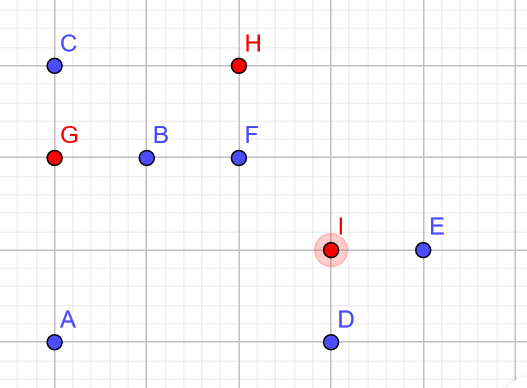
\includegraphics[height=4cm]{exemple_P_centre.png}
  \caption{Exemple du problème des 2-centres}
  \label{fig:2-Centre}
\end{figure}
La figure ci-dessus est un exemple du problème des 2-centres. Les points bleus correspondent aux points ou maison, tandis que les points rouges correspondent aux positions possibles ou placer les deux usines.
\newline
Afin de résoudre ce problème, on exprime les distances à chacune des usines sous la forme d'un tableau :
\begin{center}
\begin{tabular}{ | c | c | c | c | }
    \hline
    & G & H & I \\ \hline
    A & 2 & $\sqrt{13}$ & $\sqrt{10}$ \\ \hline
    B & 1 & $\sqrt{2}$ & $\sqrt{5}$ \\ \hline
    C & 1 & 2 & $\sqrt{13}$ \\ \hline
    D & $\sqrt{13}$ & $\sqrt{10}$ & 1 \\ \hline
    E & $\sqrt{17}$ & $2\sqrt{2}$ & 1 \\ \hline
    F & 2 & 1 & $\sqrt{2}$ \\ \hline
\end{tabular}
\end{center}
On ordonne ensuite les distances sans répétition, et on met en place un dichotomie, en cherchant un solution au problème de set-cover avec k=2, en ne considérant que les distances inférieures à celle de la dichotomie.

\subsection{Mise en place de coupe}
Afin d'assurer un temps de résolution correct, on met en place l'algorithme du simplex qui va nous permettre d'obtenir une solution dans le cadre continu et non dans le cadre discret. Afin d'affiner cette résolution, on cherche à mettre en place des coupes.

\section{Etude des coupes $\{0,\frac{1}{2}\}$ }
Avant de mettre en place la génération de coupe, j'ai étudié l'article de $\backslash$cite\{koster2009algorithms\}.

\subsection{Définition des coupes $\{0,\frac{1}{2}\}$}
On considère le problème d'optimisation linéaire dans sa forme minimiser :
$$
\left\{
    \begin{array}{ll}
        min& \ c^Tx \\
        tq &  Ax \le b \\
          & x \ge 0 \\
          & x \in Z^n \\
    \end{array}
\right.
$$
On s'interresse à une coupe de Chvatal-Gomory :
$$
\lfloor u^TA \rfloor x \le \lfloor u^Tb \rfloor, \ avec \ u \in [0,1[^m
$$
Ici, u n'évolue plus dans $[0,1[^m$, mais dans $\{0,\frac{1}{2}\}^m$.

\subsection{Existence d'une coupe}
Tout d'abord le document présente le raisonnement qui permet de déterminer si à partir d'une solution non entière le système admet un coupe, c'est à dire un vecteur u tel que l'inégalité n'est pas respectée. Pour cela, on définit une fonction de violation de la manière suivante :
$$
z(u,x^\ast)=\lfloor u^TA \rfloor x^\ast-\lfloor u^Tb \rfloor
$$
On cherche donc un vecteur u tel que $z(u,x^\ast)>0$.
Pour cela on définit les éléments suivants :
$$
\overset{\_}{A}=A \ mod \ 2, \ \overset{\_}{b}=b \ mod \ 2,\ s = b-Ax^\ast \ge 0
$$
Dans un premier temps, l'auteur énonce et fait la démonstration du lemme suivant, qui donne une condition nécessaire suffisante quand à l'existence d'une coupe :
\newline
\newline
Soit $x^\ast$ une solution entière, $\exists$ u $\in$ $\{0,\frac{1}{2}^m$ tel que $z(u,x^\ast)<0$, si et seulement si $\exists$ v $\in$ $\{0,1\}^m$ qui vérifie $v^T\overset{\_}{b}$ impair et $v^Ts+(v^T\overset{\_}{A}\ mod\ 2)x^\ast < 1 $
\newline
\newline
Pour démontrer ce lemme, il faut développer l'expression de $z(u,x^\ast)$:
\newline
\begin{equation}
\begin{split}
z(u,x^\ast) & =\lfloor u^TA \rfloor x^\ast-\lfloor u^Tb \rfloor \\
 & = \frac{1}{2}((2u^T)\overset{\_}{b}\ mod\ 2) -v^Ts-\frac{1}{2}((2u^T\overset{\_}{A}\ mod \ 2)x^\ast)
\end{split}
\end{equation}
En posant v=2u, et en remarquant que tous les termes de la différences sont positifs, on en déduit les conditions précédentes.
\newline
Ensuite, afin d'alléger la recherche d'un vecteur v adéquats, l'auteur met en place les règles de simplification suivante afin d'alléger le système sans modifier l'ensemble des coupes non-dominées.
\newline
Proposition 3:
\begin{itemize}
    \item (i) On peut supprimer les colonnes dans $\overset{\_}{A}$, qui correspondent à une valeur nulle de $x^\ast$. En effet cela ne modifie pas l'inégalité $v^Ts+(v^T\overset{\_}{A}\ mod\ 2)x^\ast < 1 $.
    \item (ii) On peut supprimer les lignes de zéro dans $(\overset{\_}{A},\overset{\_}{b})$, car cela n'a d'effet que su la slack s.
    \item (iii) On peut supprimer les colonnes de zéro de $\overset{\_}{A}$, cela ne modifie donc pas l'inégalité.
    \item (iv) On peut remplacer les colonnes identiques dans $\overset{\_}{A}$ par une seule colonne représentative, dont la variable associée est la somme des variables correspondantes. Soit aucune soit toutes les variables correspondantes devront sinon être arrondies.
    \item (v) On peut supprimer toutes colonnes unitaires de $\overset{\_}{A}$ de la forme $\overset{\_}{a}^i=e^j $ en prenant soin d'ajouter $x_i^\ast$ à $s_j$. 
    \item (vi) Toutes les colonnes dont la slack associée vérifie $s_j\ge1$ peuvent être supprimées, car sinon cela contredit directement l'inégalité si le $v_j$ correspondant vaut 1.
    \item (vii) On peut supprimer toutes les colonnes identiques dans $(\overset{\_}{A},\overset{\_}{b})$ sauf pour celle dont la slack est la plus petite.
\end{itemize}
Lors de la première itération chaque ligne du système $(\overset{\_}{A},\overset{\_}{b},s)$ correspond à une unique inégalité. Cependant pour les itérations suivantes, on doit mettre en place une opération afin de pouvoir combiner les lignes.
Si on combine les lignes i et j sur la ligne j, cette opération est la suivante :
$$
\forall k, \overset{\_}{a_{ik}}+\overset{\_}{a_{jk}}=\overset{\_}{a_{jk}} \ mod \ 2, \ \overset{\_}{b_{j}}=\overset{\_}{b_{i}}+\overset{\_}{b_{j}} \ mod \ 2, \ s_j=s_i+s_j et R_j=R_i\Delta R_j
$$
avec
$$
X\Delta Y= X\cap Y \backslash (X \cup Y)
$$
Dans le cas particulier suivant, il est possible de repérer facilement un vecteur u entraînant la violation de la coupe associée. Si on ce place dans le cas où la $i^{ème}$ rangé de $\overset{\_}{A}$ est nulle et que $\overset{\_}{b}_j = 1$, alors si $s_j<1$, en posant u tel que $\forall j \in R_j \ u_j=\frac{1}{2} $ et 0 sinon, on définit une coupe violée du système initial $(A,b,s)$. Cela se voit rapidement, en posant v tel que $\forall j \in R_j \ 1  $ et 0 sinon, et en appliquant le lemme précèdent. 
\newline
\newline
L'auteur met en place deux nouvelles propositions, qui mettent en place de nouvelles règles de simplification.
\newline
Tout d'abord, la proposition 5 est la suivante : soit i et k des indices de lignes et de colonnes tels que $\overset{\_}{a_{ik}}=1$, et $s_i=0$, alors on peut supprimer la colonne k de $\overset{\_}{A}$ à condition d'ajouter la ligne i à toutes les autres lignes telles que $\overset{\_}{a_{ik}}=1$ et en imposant $s_j=x^\ast$.
En faisant le calcul dans ce cas là, on met en avant le fait que la fonction de violation est avant et après le changement.
\newline
Enfin, la proposition 6 est la suivante : soit i et k des indices de lignes et de colonnes tels que $\overset{\_}{a_{ik}}=1$, et $s_i=0$ et $x^\ast \ge 1$, alors on peut supprimer la ligne i et la colonne k de $\overset{\_}{A}$ à condition d'ajouter la ligne i à toutes les autres lignes telles que $\overset{\_}{a_{ik}}=1$ et en imposant $s_j=x^\ast$. Pour cela on applique la proposition précédente, et on se retrouve dans la situation de la troisième proposition de suppression.
\newline
\newline
Ces règles de simplification, ainsi que de détection de coupes violées seront très utiles pour la mise en place de la méthode heuristique. 

\subsection{Pré-traitement des données}
Avant de mettre en place la recherche de coupe, un pré-traitement des données est réalisée avec les étapes suivantes : 
\begin{itemize}
    \item (a) supprimer les colonnes nulles en appliquant (3i)
    \item (b) supprimer les colonnes qui correspondent à $x^\ast$ petit en appliquant (3ii)
    \item (c) supprimer les lignes de slack supérieure ou égale à 1 en appliquant (3vi)
    \item (d) supprimer les colonnes en appliquant la proposition 5.
    \item (e) supprimer les colonnes unitaires en appliquant (3v)
    \item (f) ajouter à l'ensemble des coupes violées toute coupe correspondant à une ligne où $\overset{\_}{b}=1$ et qui à une violation d'au moins $\epsilon$, puis la supprimer de la matrice car toute coupe la contenant aura une violation inférieure
    \item (g) supprimer toutes les colonnes identiques sauf pour celle de plus petite slack
\end{itemize}
Enfin à chaque étape on prend le soin de supprimer les colonnes et lignes nulles, ainsi que les lignes de slack supérieure à 1 dans $(\overset{\_}{A},\overset{\_}{b})$.

\subsection{Méthode avec un programme linéaire}
Une première approche peut-être de modéliser le problème de coupe par un système linéaire de la forme suivante :
$$
\left\{
    \begin{array}{ll}
        z=&min \ s^Tv+(x^\ast)^Ty \\
        tq &  \overset{\_}{b}^Tv-2q=1 \\
          & \overset{\_}{A}^Tv-2r-y=0 \\
          & v \in \{0,1\}^n \\
          & y \in \{0,1\}^n \\
          & r \in Z^n_+ \\
          & q \in Z^n \\
    \end{array}
\right.
$$
La première égalité impose que $\overset{\_}{b}^Tv$ soit impair, la seconde permet de calculer le reste de la division euclidienne de $\overset{\_}{A}^Tv$ par 2. La fonction coût permet de déterminer $v^Ts+(v^T\overset{\_}{A}\ mod\ 2)x^\ast$. Si cette valeur est inférieure ou égale à 1 alors une coupe violée n'a pas été trouvée, et si cette valeur est supérieure à 1 alors il en existe une coupe violée, qui correspond à la combinaison des inégalités pour laquelle $v_j$ vaut 1.
Cependant, on peut s'attendre à ce que le temps de résolution de ce programme auxiliaire soit trop long, il est donc intéressant d'étudier les méthodes de résolution heuristique.

\subsection{Méthode heuristique}
La méthode de résolution heuristique suivante est développée. Tant que l'on ne trouve pas de coupe violée, on teste les combinaisons de plus en plus grande d'inégalité.
De plus les données sont pré-traitées afin d'accélérer la vitesse de résolution.

\subsection{Résultat et performance des différentes méthodes}

\subsubsection{Résultat du pré-traitement des données}

Les tests ont été réalisés sur tous les noeuds du branch\&cut, sans imposer de violation minimun.
Les étapes (a) à (c) réduisent la taille de $\overset{\_}{A}$ d'en moyenne 83,2\%, allant de 46,96\% jusqu'à 99,9\%.
Après applications des étapes (a) à (c), on étudie les résultats des étapes suivantes en fonction de la taille actuelle de la matrice $\overset{\_}{A}$. Les étapes (d) et (e) simplifient le système de 1,26\% et 1,5\% en supprimant respectivement les colonnes unitaires et les lignes nulles qui contiennent une coupe violée et enfin on peut supprimer 40,7\% en supprimant les colonnes identiques.
On obtient alors en considérant chacune des étapes une simplification de 95,5\% en moyenne.
Cette simplification est très significative et permet d'accélerer grandement le temps de résolution, et permet de résoudre en moins de 10s des instances qui ne pouvaient sinon pas être résolues en dessous de ce temps.

\subsubsection{Comparaison du nombre de noeuds du branche\&cut}
Un premier élément pour comparer les performances de la coupe $\{0,\frac{1}{2}\}$, et la mesure du nombre de noeuds dans le branch\&cut. Dans cet approche, on compare 3 éléments :
\begin{itemize}
    \item Fischetti et Lotti font appel à la coupe de Chvatal-Gomory pour la séparation
    \item SCIP par défaut
    \item SCIP en remplaçant le séparateur standard avec la coupe $\{0,\frac{1}{2}\}$, en ajoutant à chaque fois que la coupe la plus violée.
\end{itemize}
Par rapport à Fischetti et Lotti, 40\% de coupe en moins sont réalisées. Cependant le SCIP réalise en général plus d'un branch\&cut, on est donc amenée en général à réaliser plus de coupes.
En considérant la méthode faisant appel au programme linéaire auxiliaire, et en ajoutant les coupes violées ne jouant pas un rôle dans la coupe optimale, on arrive à diminuer de 26\% en général le nombre de noeuds dans le branch\&cut. Cepedant ceux-ci évoluent de moins 84\% à plus 158\%. En outre, on atteint ce résultat en sacrifiant le temps de calcul. En effet on voit une augmentation de plus 158\% au temps de calcul.
Une telle approche du problème n'est donc pas adaptée, et on va choisir de comparer plutôt le temps CPU.

\subsubsection{Comparaison du temps CPU}
Afin de mettre en évidence que la résolution faisant appel un programme linéaire auxiliaire n'est pas adaptée, on va comparer le temps de résolution des 3 éléments suivants :
\begin{itemize}
    \item le SCIP par défaut
    \item le SCIP faisant appel au programme linéaire auxiliaire 
    \item le SCIP faisant appel à la méthode heuristique
\end{itemize}
De plus, on ne considère pas toutes les coupes violées, seulement celle dont la fonction de violation est supérieure à 0.35 afin d'éviter de générer des coupes inefficaces. Ensuite, jusqu'à 100 coupes violées sont transmises au SCIP, qui va choisir de les prendre en compte ou non.
La méthodes heuristique améliore de 7\% en moyenne sur toutes les instances le temps de résolution de l'algorithme, et de 21\% pour les instances dont le temps de résolution absolue plus grand que 10s avec le SCIP par défault.
\newline
On remarque bien que la résolution heuristique semble la plus adaptée.

\addcontentsline{toc}{chapter}{Bibliographie}

%% Feuille de style bibliographique : monjfm.bst
\bibliographystyle{apalike}
\bibliography{bibliography}

\end{document}
